\documentclass[leqno]{article}
\usepackage[utf8]{inputenc}
\usepackage[T1]{fontenc}
\usepackage{amsfonts}
\usepackage{fourier}
\usepackage{heuristica}
\usepackage{enumerate}
\author{Colin Roberts}
\title{MATH 570, Homework 7}
\usepackage[left=3cm,right=3cm,top=3cm,bottom=3cm]{geometry}
\usepackage{amsmath}
\usepackage[thmmarks, amsmath, thref]{ntheorem}
%\usepackage{kbordermatrix}
\usepackage{mathtools}
\usepackage{tikz-cd}
\usepackage{ragged2e}

\theoremstyle{nonumberplain}
\theoremheaderfont{\itshape}
\theorembodyfont{\upshape:}
\theoremseparator{.}
\theoremsymbol{\ensuremath{\square}}
\newtheorem{proof}{Proof}
\theoremsymbol{\ensuremath{\square}}
\newtheorem{lemma}{Lemma}
\theoremsymbol{\ensuremath{\blacksquare}}
\newtheorem{solution}{Solution}
\theoremseparator{. ---}
\theoremsymbol{\mbox{\texttt{;o)}}}
\newtheorem{varsol}{Solution (variant)}

\newcommand{\tr}{\mathrm{tr}}
\newcommand{\Int}{\ensuremath{\mathrm{Int}}}
\newcommand{\N}{\ensuremath{\mathbb{N}}}
\newcommand{\Q}{\ensuremath{\mathbb{Q}}}
\newcommand{\R}{\ensuremath{\mathbb{R}}}
\newcommand{\Z}{\ensuremath{\mathbb{Z}}}
\newcommand{\cB}{\ensuremath{\mathcal{B}}}
\newcommand{\cF}{\ensuremath{\mathcal{F}}}
\newcommand{\obj}{\ensuremath{\mathrm{Obj}}}


\begin{document}
\maketitle
\begin{large}
\begin{center}
Solutions
\end{center}
\end{large}
\pagebreak

%%%%%%%%%%%%%%%%%%%%%%%%%%%%%%%%%%%%%%%%%%%%%%%%%%%%%%%%%%%%%%%%%%%%%%%%%%%%%%%%%%%%%%%%%%%%%%%%%%%%%%%%%%%%%%%%%%%%%
%%%%%%%%%%%%%%%%%%%%%%%%%PROBLEM 1%%%%%%%%%%%%%%%%%%%%%%%%%%%%%%%%%%%%%%%%%%%%%%%%%%%%%%%%%%%%%%%%%%%%%%%%%%%%%%%%%%%%%%%%%%%%%%%%%%%%%%%%%%%%%%%%%%%%%%%%%%%%%%%%%%%%%%%%%%%%%%%%%%%%%%%%%%%%%%%%%%%%%%%%%%%%%%%%%%%%%%%%%%%%%%%%%%%%%%%%

\noindent\textbf{Problem 1.}  Suppose $f,g\colon S^n\to S^n$ are continuous maps such that $f(x)\neq -g(x)$ for any $x\in S^n$. Prove that $f$ and $g$ are homotopic.

\emph{Hint: As an easier case, what if we instead had $f,g\colon S^n\to \R^{n+1}\setminus\{\vec{0}\}$ with the the line segment from $f(x)$ to $g(x)$ not passing through the origin for all $x\in S^n$? Can you modify a proof of this easier case to handle the problem above where $f,g\colon S^n\to S^n$ with $f(x)\neq -g(x)$?}

\noindent\rule[0.5ex]{\linewidth}{1pt}

\begin{proof}
Consider the hint.  We have, since no line segment between $f(x)$ and $g(x)$ will pass through $0$, that there is a straight line homotopy between $f(x)$ and $g(x)$.  In order to make this work for $f,g\colon S^n \to S^n$ instead of $f,g \colon S^n \to \R\setminus \{0\}$ we have the homotopy given by
\[
H(x,t)=\frac{(1-t)f(x)+tg(x)}{\|(1-t)f(x)+tg(x)\|}.
\]
Note that $H(\cdot,0)=f$ and $H(\cdot, 1)=g$.  This is a continuous homotopy since the denominator is never zero, and the numerator is addition of continuous functions.
\end{proof}

\pagebreak

%%%%%%%%%%%%%%%%%%%%%%%%%%%%%%%%%%%%%%%%%%%%%%%%%%%%%%%%%%%%%%%%%%%%%%%%%%%%%%%%%%%%%%%%%%%%%%%%%%%%%%%%%%%%%%%%%%%%%
%%%%%%%%%%%%%%%%%%%%%%%%%PROBLEM 2%%%%%%%%%%%%%%%%%%%%%%%%%%%%%%%%%%%%%%%%%%%%%%%%%%%%%%%%%%%%%%%%%%%%%%%%%%%%%%%%%%%%%%%%%%%%%%%%%%%%%%%%%%%%%%%%%%%%%%%%%%%%%%%%%%%%%%%%%%%%%%%%%%%%%%%%%%%%%%%%%%%%%%%%%%%%%%%%%%%%%%%%%%%%%%%%%%%%%%%%


\noindent\textbf{Problem 2.} Let $X$ be a topological space and let $g$ be a path in $X$ from $p$ to $q$. Let $\Phi_g\colon\pi_1(X,p)\to\pi_1(X,q)$ denote the group isomorphism defined in Theorem~7.13.

If $h\colon X\to Y$ is continuous, then show that the following diagram commutes:
\begin{center}
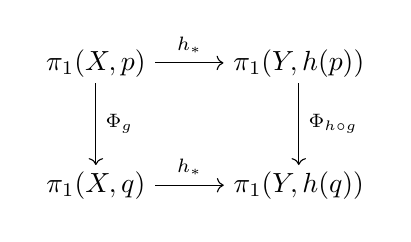
\begin{tikzpicture}[description/.style={fill=white,inner sep=2pt}] 
\matrix (m) [matrix of math nodes, row sep=3em, 
column sep=2.5em, text height=1.5ex, text depth=0.25ex] 
{  
\pi_1(X,p) & \pi_1(Y,h(p)) \\
\pi_1(X,q)	& \pi_1(Y,h(q)) \\
};
;
\path[->,font=\scriptsize]
(m-1-1) edge node[auto] {$h_*$} (m-1-2)
(m-1-1) edge node[auto] {$\Phi_g$} (m-2-1)
(m-2-1) edge node[auto] {$h_*$} (m-2-2)
(m-1-2) edge node[auto] {$\Phi_{h\circ g}$} (m-2-2)
;
\end{tikzpicture}
\end{center}


\noindent\rule[0.5ex]{\linewidth}{1pt}

\begin{proof}
To show that this diagram commutes we need to show that for $[f]\in \pi_1 (X,p)$ that $\phi_{h\circ g} \circ h_* [f]=\phi_g \circ h_* [f]$. First we show that $\overline{h\circ g} = h \circ \overline{g}$.  We have
\begin{align*}
\overline{h\circ g}(t)&=h\circ g (1-t)\\
&= h \circ \overline{g}(t).
\end{align*}
Then
\begin{align*}
\phi_{h\circ g} \circ h_* [f] &= \phi_{h\circ g} [h\circ f]\\
&= [\overline{(h\circ g}]\cdot (h\circ f) \cdot (h\circ g)]\\
&= [(h\circ \overline{g})\cdot (h\circ f) \cdot (h\circ g)]\\
&= [h \circ (\overline{g} \cdot f \cdot g)]\\
&= h_* [\overline{g} \cdot f \cdot g]\\
&= h_* \circ [\overline{g}][f][g]\\
&= h_* \circ \phi_g [f].
\end{align*}
Thus the diagram commutes.
\end{proof}


\pagebreak


%%%%%%%%%%%%%%%%%%%%%%%%%%%%%%%%%%%%%%%%%%%%%%%%%%%%%%%%%%%%%%%%%%%%%%%%%%%%%%%%%%%%%%%%%%%%%%%%%%%%%%%%%%%%%%%%%%%%%
%%%%%%%%%%%%%%%%%%%%%%%%%PROBLEM 3%%%%%%%%%%%%%%%%%%%%%%%%%%%%%%%%%%%%%%%%%%%%%%%%%%%%%%%%%%%%%%%%%%%%%%%%%%%%%%%%%%%%%%%%%%%%%%%%%%%%%%%%%%%%%%%%%%%%%%%%%%%%%%%%%%%%%%%%%%%%%%%%%%%%%%%%%%%%%%%%%%%%%%%%%%%%%%%%%%%%%%%%%%%%%%%%%%%%%%%%


\noindent\textbf{Problem 3.} Let $X$ be a path-connected topological space, and let $p,q\in X$. Show that $\pi_1(X,p)$ is abelian if and only if for any two paths $g,g'$ from $p$ to $q$ in $X$, we have $\Phi_g=\Phi_{g'}$ (as isomorphisms from $\pi_1(X,p)$ to $\pi_1(X,q)$). 

\noindent\rule[0.5ex]{\linewidth}{1pt}

\begin{proof} 
First, suppose that $\pi_1 (X,p)$ is abelian.  Denote the constant path in $\pi_1 (X,p)$ by $[C_p]$. Then for $[f]\in \pi_1 (X,p)$ we have
\begin{align*}
\Phi_g [f] &= [\overline{g}] [f] [g]\\
&= [\overline{g}][g][f]\\
&= [C_p][f]\\
&= [\overline{g'}][g'][f]\\
&= [\overline{g'}][f][g']\\
&= \Phi_{g'} [f].
\end{align*}
So we have that $\Phi_g = \Phi_{g'}$.

For the converse, suppose that we have $\Phi_g = \Phi_{g'}$. Then
\begin{align*}
\Phi_g [f] &= [\overline{g}][f][g]\\
&= \Phi_{C_p} [f] && \textrm{since the above is just homotopy equivalent to this}\\
\implies [f]&=[\overline{g}][f][g].
\end{align*}
Which implies that $\pi_1 (X,p)$ is abelian.
\end{proof}


\pagebreak



%%%%%%%%%%%%%%%%%%%%%%%%%%%%%%%%%%%%%%%%%%%%%%%%%%%%%%%%%%%%%%%%%%%%%%%%%%%%%%%%%%%%%%%%%%%%%%%%%%%%%%%%%%%%%%%%%%%%%
%%%%%%%%%%%%%%%%%%%%%%%%%PROBLEM 4%%%%%%%%%%%%%%%%%%%%%%%%%%%%%%%%%%%%%%%%%%%%%%%%%%%%%%%%%%%%%%%%%%%%%%%%%%%%%%%%%%%%%%%%%%%%%%%%%%%%%%%%%%%%%%%%%%%%%%%%%%%%%%%%%%%%%%%%%%%%%%%%%%%%%%%%%%%%%%%%%%%%%%%%%%%%%%%%%%%%%%%%%%%%%%%%%%%%%%%%


\noindent\textbf{Problem 4.} Let $F\colon C\to D$ be a (covariant) functor from category $C$ to category $D$. Prove that if $X,Y\in\obj(C)$ are isomorphic objects in $C$, then $F(X),F(Y)$ are isomorphic objects in $D$. 

\noindent\rule[0.5ex]{\linewidth}{1pt}

\begin{proof}
The following diagram will prove useful (at least in my visualization):
\begin{center}
\[
\begin{tikzcd}
X \arrow[dd, "F"'] \arrow[rr, "\varphi", bend left] &  & Y \arrow[dd, "F"] \arrow[ll, "\varphi^{-1}"] \\
 &  &  \\
F(X) \arrow[rr, "F(\varphi)"] &  & F(Y) \arrow[ll, "F(\varphi^{-1})", bend left]
\end{tikzcd}
\]
\end{center}

Since $X$ and $Y$ are isomorphic in $\mathrm{Obj}(C)$ we have that $\varphi \colon X \to Y$ is an isomorphism with inverse $\varphi^{-1}$.  Then we have that $F(\mathrm{Id_X}) = F(\varphi^{-1} \circ \varphi) = F(\varphi^{-1}) \circ F(\varphi) = \mathrm{Id}_{F(X)}$.  This means that $F(\varphi)$ is an isomorphism $F(\varphi) \colon F(X) \to F(Y)$ with inverse $F(\varphi^{-1})$ and we have that $F(X)$ and $F(Y)$ are isomorphic objects in $\mathrm{Obj}(D)$.
\end{proof}


\pagebreak


%%%%%%%%%%%%%%%%%%%%%%%%%%%%%%%%%%%%%%%%%%%%%%%%%%%%%%%%%%%%%%%%%%%%%%%%%%%%%%%%%%%%%%%%%%%%%%%%%%%%%%%%%%%%%%%%%%%%%
%%%%%%%%%%%%%%%%%%%%%%%%%PROBLEM 5%%%%%%%%%%%%%%%%%%%%%%%%%%%%%%%%%%%%%%%%%%%%%%%%%%%%%%%%%%%%%%%%%%%%%%%%%%%%%%%%%%%%%%%%%%%%%%%%%%%%%%%%%%%%%%%%%%%%%%%%%%%%%%%%%%%%%%%%%%%%%%%%%%%%%%%%%%%%%%%%%%%%%%%%%%%%%%%%%%%%%%%%%%%%%%%%%%%%%%%%


\noindent\textbf{Problem 5.} Let $X$ be a toplogical space. Prove that the following statements are equivalent:
\begin{enumerate}
\item[(i)] $X$ is compact.
\item[(ii)] For every collection $\{C_\alpha\}_{\alpha\in A}$ of closed subsets of $X$ with $\cap_{\alpha\in A} C_\alpha=\emptyset$, there is a finite subcollection $\{C_{\alpha_1},\ldots,C_{\alpha_n}\}$ with $C_{\alpha_1}\cap\ldots\cap C_{\alpha_n}=\emptyset$.
\end{enumerate}

\noindent\rule[0.5ex]{\linewidth}{1pt}

\begin{proof}
To show equivalence we prove that (i) implies (ii) and (ii) implies (i).  

For the first implication, suppose that $X$ is compact. Then let $\{C_\alpha\}_{\alpha \in A}$ be a collection of closed subsets so that $\cap_{\alpha} C_\alpha=\emptyset$. Then we have that $X\setminus (\cap_{\alpha} C_\alpha)=\cup_\alpha X\setminus C_\alpha = X$.  Thus we have that $\cup_\alpha X\setminus C_\alpha$ is an open cover of $X$ and by compactness we have that there exists a finite subcover. Put $\cup_{i=1}^n X\setminus C_{\alpha_i}$ as our finite subcover and note that $X\setminus (\cup_{i=1}^n X\setminus C_{\alpha_i}) = \cap_{i=1}^n C_{\alpha_i} = \emptyset$. 

For the second implication, suppose that for every collection of closed subsets $\{C_\alpha\}_{\alpha \in A}$ satisfying $\cap_{\alpha} C_\alpha = \emptyset$ we have $\cap_{i=1}^n C_{\alpha_i} = \emptyset$. Note that $\cup_\alpha X\setminus C_\alpha$ is an arbitrary open cover and $X\setminus (\cap_{i=1}^n C_{\alpha_i})=\cup_{i=1}^n X\setminus C_{\alpha_i}$ is a finite subcover. So $X$ is compact.
\end{proof}


\pagebreak



\end{document}

